\documentclass[10pt]{article}
\usepackage{amsmath,amsfonts,times}
\usepackage{graphicx,color,tikz}
\usepackage[paperwidth=17.6cm,paperheight=11.3cm,lmargin=0in,rmargin=0in,tmargin=0.in,bmargin=0.in]{geometry}
\usepackage{bm}
\usetikzlibrary{arrows.meta,shadows,positioning,calc,backgrounds}

% One colour per piece of the search the caller supplies.
\definecolor{cquery}{rgb}{0.10,0.35,0.80}
\definecolor{cbound}{rgb}{0.80,0.10,0.10}
\definecolor{cvisit}{rgb}{0.90,0.50,0.00}
\definecolor{corder}{rgb}{0.50,0.20,0.65}
\definecolor{cleaf}{rgb}{0.05,0.55,0.20}

\tikzset{
  node/.style={draw=black, minimum width=9mm, minimum height=7mm, rectangle, very thick, fill=white, drop shadow, rounded corners=4pt, font=\small},
  pruned/.style={node, draw=black!35, text=black!35, fill=black!4, drop shadow={opacity=0.1}},
  edge/.style={thick, draw=black},
  prunededge/.style={thick, draw=black!30, densely dashed},
  key/.style={font=\scriptsize, fill=white, inner sep=1pt},
  walk/.style={-{Stealth[length=2.5mm]}, line width=1.3pt, draw=cquery!70, rounded corners=6pt},
  event/.style={circle, draw=black, fill=yellow!40, inner sep=1pt, minimum width=4.6mm, font=\scriptsize\bfseries},
  cross/.style={cbound, line width=1.6pt, opacity=0.55},
}

\begin{document}
\nopagecolor
\centering
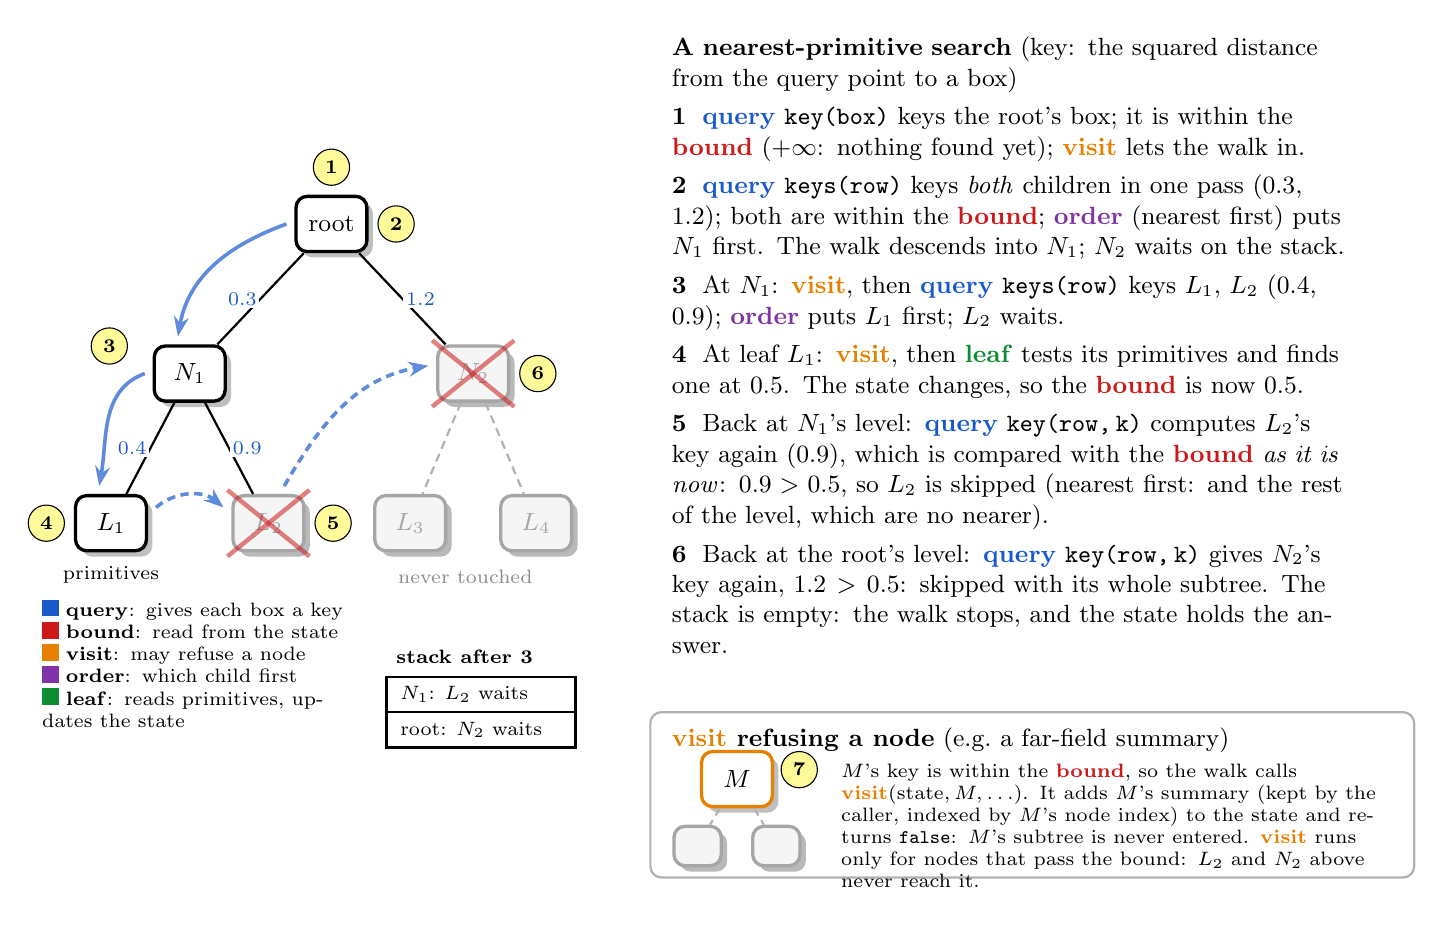
\begin{tikzpicture}[x=1cm, y=1cm]

  % ── The tree: a root, two interior nodes, four leaves (K = 2 here; the walk is the same at any K).
  \node[node]   (R)  at (3.6, 6.9) {root};
  \node[node]   (N1) at (1.8, 5.0) {$N_1$};
  \node[pruned] (N2) at (5.4, 5.0) {$N_2$};
  \node[node]   (L1) at (0.8, 3.1) {$L_1$};
  \node[pruned] (L2) at (2.8, 3.1) {$L_2$};
  \node[pruned] (L3) at (4.6, 3.1) {$L_3$};
  \node[pruned] (L4) at (6.2, 3.1) {$L_4$};

  \draw[edge]       (R)  -- node[key, left]  {\color{cquery}$0.3$} (N1);
  \draw[edge]       (R)  -- node[key, right] {\color{cquery}$1.2$} (N2);
  \draw[edge]       (N1) -- node[key, left]  {\color{cquery}$0.4$} (L1);
  \draw[edge]       (N1) -- node[key, right] {\color{cquery}$0.9$} (L2);
  \draw[prunededge] (N2) -- (L3);
  \draw[prunededge] (N2) -- (L4);

  % The primitives in leaf L1, and the subtree never touched.
  \node[font=\scriptsize, below=0.5mm of L1] {primitives};
  \node[font=\scriptsize, text=black!45, below=1.0mm of L3, xshift=7mm] {never touched};

  % Pruned nodes, crossed out.
  \foreach \n in {L2, N2} {
    \draw[cross] ($(\n.north west)+(-0.05,0.05)$) -- ($(\n.south east)+(0.05,-0.05)$);
    \draw[cross] ($(\n.north east)+(0.05,0.05)$) -- ($(\n.south west)+(-0.05,-0.05)$);
  }

  % ── The walk, as a path through the tree.
  \draw[walk] ($(R.west)+(-0.1,0)$) to[out=200, in=80] ($(N1.north)+(-0.15,0.1)$);
  \draw[walk] ($(N1.west)+(-0.1,0)$) to[out=200, in=80] ($(L1.north)+(-0.15,0.1)$);
  \draw[walk, densely dashed] ($(L1.east)+(0.1,0.2)$) to[out=40, in=140] ($(L2.west)+(-0.1,0.2)$);
  \draw[walk, densely dashed] ($(L2.north)+(0.2,0.1)$) to[out=60, in=190] ($(N2.west)+(-0.1,0.1)$);

  % ── Numbered events where the walk calls the caller's pieces.
  \node[event] at ($(R.north)+(0,0.35)$) {1};
  \node[event] at ($(R.east)+(0.35,0)$) {2};
  \node[event] at ($(N1.west)+(-0.55,0.35)$) {3};
  \node[event] at ($(L1.west)+(-0.35,0)$) {4};
  \node[event] at ($(L2.east)+(0.35,0)$) {5};
  \node[event] at ($(N2.east)+(0.35,0)$) {6};

  % ── The stack after event 3: one entry per level, holding the children still to visit.
  \begin{scope}[shift={(4.3,0.25)}]
    \node[font=\scriptsize\bfseries, anchor=west] at (0,1.15) {stack after 3};
    \draw[thick] (0,0) rectangle (2.4,0.45);
    \draw[thick] (0,0.45) rectangle (2.4,0.9);
    \node[font=\scriptsize, anchor=west] at (0.05,0.225) {root: $N_2$ waits};
    \node[font=\scriptsize, anchor=west] at (0.05,0.675) {$N_1$: $L_2$ waits};
  \end{scope}

  % ── Which colour is which piece.
  \node[anchor=north west, font=\scriptsize, text width=4.1cm, align=left] at (-0.2,2.25) {%
    \textcolor{cquery}{\rule{6pt}{6pt}}~\textbf{query}: gives each box a key\\
    \textcolor{cbound}{\rule{6pt}{6pt}}~\textbf{bound}: read from the state\\
    \textcolor{cvisit}{\rule{6pt}{6pt}}~\textbf{visit}: may refuse a node\\
    \textcolor{corder}{\rule{6pt}{6pt}}~\textbf{order}: which child first\\
    \textcolor{cleaf}{\rule{6pt}{6pt}}~\textbf{leaf}: reads primitives, updates the state%
  };

  % ── The events, and which piece runs at each.
  \begin{scope}[shift={(7.7,0)}]
    \node[anchor=north west, text width=8.6cm, font=\small, align=left] at (0.1,9.4) {%
      \textbf{A nearest-primitive search} (key: the squared distance from the query point to a box)\\[3pt]
      \textbf{1}\; \textcolor{cquery}{\textbf{query}} \texttt{key(box)} keys the root's box; it is within the \textcolor{cbound}{\textbf{bound}} ($+\infty$: nothing found yet); \textcolor{cvisit}{\textbf{visit}} lets the walk in.\\[3pt]
      \textbf{2}\; \textcolor{cquery}{\textbf{query}} \texttt{keys(row)} keys \emph{both} children in one pass ($0.3$, $1.2$); both are within the \textcolor{cbound}{\textbf{bound}}; \textcolor{corder}{\textbf{order}} (nearest first) puts $N_1$ first. The walk descends into $N_1$; $N_2$ waits on the stack.\\[3pt]
      \textbf{3}\; At $N_1$: \textcolor{cvisit}{\textbf{visit}}, then \textcolor{cquery}{\textbf{query}} \texttt{keys(row)} keys $L_1$, $L_2$ ($0.4$, $0.9$); \textcolor{corder}{\textbf{order}} puts $L_1$ first; $L_2$ waits.\\[3pt]
      \textbf{4}\; At leaf $L_1$: \textcolor{cvisit}{\textbf{visit}}, then \textcolor{cleaf}{\textbf{leaf}} tests its primitives and finds one at $0.5$. The state changes, so the \textcolor{cbound}{\textbf{bound}} is now $0.5$.\\[3pt]
      \textbf{5}\; Back at $N_1$'s level: \textcolor{cquery}{\textbf{query}} \texttt{key(row,\,k)} computes $L_2$'s key again ($0.9$), which is compared with the \textcolor{cbound}{\textbf{bound}} \emph{as it is now}: $0.9 > 0.5$, so $L_2$ is skipped (nearest first: and the rest of the level, which are no nearer).\\[3pt]
      \textbf{6}\; Back at the root's level: \textcolor{cquery}{\textbf{query}} \texttt{key(row,\,k)} gives $N_2$'s key again, $1.2 > 0.5$: skipped with its whole subtree. The stack is empty: the walk stops, and the state holds the answer.%
    };
  \end{scope}

  % ── A second panel: visit refusing a node.
  \begin{scope}[shift={(7.8,-1.25)}]
    \draw[black!30, thick, rounded corners=4pt] (-0.15,-0.15) rectangle (9.55,1.95);
    \node[anchor=north west, font=\small] at (0,1.88) {\textbf{\textcolor{cvisit}{visit} refusing a node} (e.g.\ a far-field summary)};
    \node[node, draw=cvisit] (M) at (0.95,1.1) {$M$};
    \node[pruned, minimum width=6mm, minimum height=5mm] (M1) at (0.45,0.25) {};
    \node[pruned, minimum width=6mm, minimum height=5mm] (M2) at (1.45,0.25) {};
    \draw[prunededge] (M) -- (M1);
    \draw[prunededge] (M) -- (M2);
    \node[event] at ($(M.east)+(0.32,0.12)$) {7};
    \node[anchor=north west, text width=7.1cm, font=\scriptsize, align=left] at (2.15,1.42) {%
      $M$'s key is within the \textcolor{cbound}{\textbf{bound}}, so the walk calls \textcolor{cvisit}{\textbf{visit}}$(\text{state}, M, \ldots)$. It adds $M$'s summary (kept by the caller, indexed by $M$'s node index) to the state and returns \texttt{false}: $M$'s subtree is never entered. \textcolor{cvisit}{\textbf{visit}} runs only for nodes that pass the bound: $L_2$ and $N_2$ above never reach it.%
    };
  \end{scope}

\end{tikzpicture}

\end{document}
